\section{Speculative Execution}
Speculative execution is a technique implemented by the majority of modern CPUs to maximize perfomances. 
As the name suggests, it is based on the execution of operations that might or might not be performed. The entity that predicts wether or not a certain instruction path, called branch, will be taken is called Branch Predictor.

\subsection{Branch Prediction}
A signifcant number of implementations of branch prediction have been designed over the last 50 years, many of which are the evolution of previously designed 
For the sake of this paper we will just differentiate between 2 of them, more precisely 2 macro-categories of branch prediction.
\subsubsection{Static Branch Prediction}
Static Branch Prediction is the simplest type of Branch Prediction. Predictor behaviour does not change during the execution of a program. The simplest examples are predictors that either predict that branch are always taken or always not taken. Some ISAs give the possibility, when using branch instructions, to insert a bit that hints wether a branch should be predicted taken or not.
\subsubsection{Dynamic Branch Prediction}
Dynamic Branch Predictors change behaviour according to information gathered at run-time, for an improved misprediction rate. 

\subsection{Branch Target Prediction}
Another type of speculation implemented in modern CPUs is Branch Target Prediction.
Indirect jumps are jump instructions where the target address is not directly passed, a register or a memory address containing the target is given instead.
This means that once the CU decodes the indirect jump instruction, clock cycles are spent to fetch the address from the register, cache or, worst-case scenario, a cache-miss happens and the target is fetched from main memory.
To fasten up this process, in order to fetch the target instruction as soon as possible, modern CPUs implement what's called a Branch Target Predictor.
Branch Target Predictor uses a buffer called BTB(Branch Target Buffer), which structure is analog to a cache: it associates instruction PCs to branch target PCs. Every time a new indirect jump is fetch and decoded, its PC and target address are stored in the BTB.
For every entry in the table 2 predictions bits are added, just like branch prediction 2-bit schema, to improve target prediction.
This means that new entry have 2 prediction bits set as 'Predict Taken'.
Every time an instruction is fetched, the BTB is looked up to check if it contains the instruction PC, if so, then the associated target address is sent out.
If it target turns out to be correct ...
If not the entry is deleted from the BTB, and 2 cycles are lost.
If the instruction PC is not in the BTB, if after being decoded turns it's an jump instruction then its PC and target address are saved in the table.
Workflow can be seen in Figure underneath:
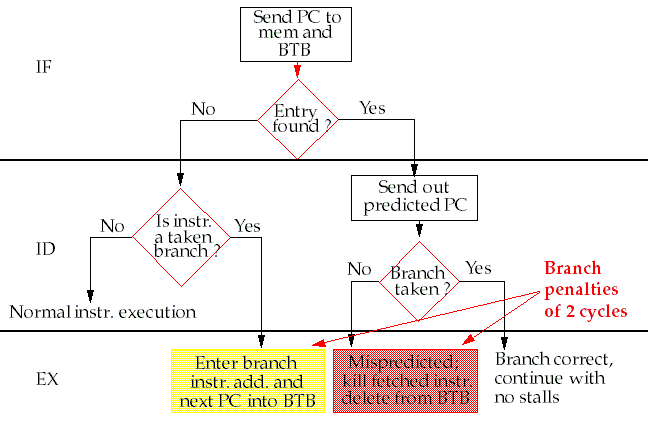
\includegraphics[scale=0.35]{img/BTB.png}

\subsection{Return Stack Buffer}

\subsection{Store Buffer}
